
\documentclass[usenatbib]{mnras}

\usepackage{newtxtext,newtxmath}
\usepackage[T1]{fontenc}

\DeclareRobustCommand{\VAN}[3]{#2}
\let\VANthebibliography\thebibliography
\def\thebibliography{\DeclareRobustCommand{\VAN}[3]{##3}\VANthebibliography}


%%%%% AUTHORS - PLACE YOUR OWN PACKAGES HERE %%%%%


\usepackage{graphicx}
\usepackage{amsmath}

\title{Tidal Evolution of M33’s Dark Matter Halo}

\author{
Aidan DeBrae$^{1}$
\\
% List of institutions
$^{1}$Department of Astronomy, University of Arizona, 933 North Cherry Avenue, Tucson, AZ, 85719}

% Don't change these lines
\begin{document}
\label{firstpage}
\pagerange{\pageref{firstpage}--\pageref{lastpage}}
\maketitle

\begin{abstract}
    The shape of the DM halo is an important feature when analyzing galaxy evolution. In this paper I focus on the shape of M31's satellite halo, M33. The primary interest to understand how the shape changes as the MW and M31 move toward collision and eventual merger. The results show that the halo begins with a triaxial shape which evolves to being oblate during the apocenter approach. The oblateness is further extended during the pericenter approach.  
\end{abstract}
% Select between one and six entries from the list of approved keywords.
% Don't make up new ones.
\begin{keywords}
Local Group -- Dark Matter Halo -- Galaxy Merger -- Cold Dark Matter Theory -- Satellite Galaxy -- Halo Shape -- Hernquist Profile
\end{keywords}

%%%%%%%%%%%%%%%%%%%%%%%%%%%%%%%%%%%%%%%%%%%%%%%%%%

%%%%%%%%%%%%%%%%% BODY OF PAPER %%%%%%%%%%%%%%%%%%

\section{Introduction}
Observations of our cosmic structure continually present evidence which further support the theoretical model that indicates our universe is primarily composed of Dark Matter (DM). Although there are many theories about what dark matter could actually be it is generally concluded it is a source of matter which has little to no interaction with baryonic matter except through gravity. Almost all of the evidence which supports the the presence of DM comes from observing the structure and behavior of galaxies. A particularly strong piece of observational evidence for dark matter is the affect of gravitational lensing. Due to their immense gravitational potential galaxies are capable of distorting light such that we can use the curvature of the light to calculate the mass of the galaxy. \citep{Massey_2010}. The results consistently show that galaxies contain significantly more mass than just the observed baryonic matter. This is further supported by physical characteristics of the galaxy like the rotation curve. Measurements of rotation curves indicate the presence of dark matter because rather than a bell shaped distribution in which the rotational velocity displays a peak and then falls off toward the edge of the galaxy the curve exhibits a nearly flat velocity distribution throughout the majority of the galaxy \citep{Hoeneisen19}. This indicates there is a very large source of mass which extends beyond the edges of the halo. It is important to consider the potential consequences of the influence of dark matter halos. The evidence clearly proves the effects of dark matter halos can dramatically impact the physical characteristics of a galaxy. It would thus be reasonable to conclude DM might influence other properties of the galaxy like orbital kinematics, star formation, and even the super massive black hole at the center of the galaxy \citep{Springel05}. If the dark matter halo is expected to play such an important role in galactic evolution it is critical to investigate the the structure and behavior of the halo. Conveniently, observations have allowed astrophysicists to determine the fate of the Local Group system which might provide some understanding of how dark matter behaves. In roughly 4 billion years the Local Group will experience a catastrophic event. That event is when our own galaxy, the Milky Way (MW), will collide with our closest neighboring galaxy, Andromeda (M31). The collision of these two galaxies will produce immense changes to their own structure as well as any nearby satellite galaxies. It follows that the dark matter halos which surround these galaxies will also undergo immense changes. Using simulations, an analysis of the shape and density profile of the halos as this collision event occurs will offer insight into how the structure of the halo changes over time. 


To investigate the relationship between galaxies and their dark matter halos it is best to first carefully define the broad terms associated with them. A galaxy is defined by \cite{Willman12} as ``[...] a gravitationally bound set of stars whose properties cannot be explained by a combination of baryons (gas \& stars) and Newton's laws of gravity.'' Due to the complexity of galaxy evolution it is quite difficult to precisely define what it means. An excellent general description is provided by \cite{Mo10} where galaxy evolution is defined by "[...] comparing [galaxy] properties, in a statistical sense, at different epochs." This definition motivates the exploration of the Local Group dark matter halos since it has been firmly established by observations that dark matter plays an important role in determining the properties of the galaxy it surrounds. Additionally, the collision of the MW \& M31 in the future provides a tightly constrained system in which the properties of the galaxies and their halos can be constructed in N-body simulations to predict how both the individual galaxies and the Local Group will evolve over time. Simulations have shown that the properties of dark matter effect the morphology of galaxies over time \citep{Cataldi21}. This is further accentuated by \cite{Chua22} as their research concluded there is a strong relationship between the properties of the halo shape and baryonic matter stating, ``[...] the change in halo shape depends on aspects of the baryonic physics; e.g. gas cooling, star formation and galactic feedback.'' Thus, understanding the shape of a halo is vital in developing a clear picture of the relationship between a galaxy and it's surrounding dark matter halo. Research indicates the galaxy-halo relationship plays an important role in galactic evolution.     


Most research analyzing the shape of dark matter halos has been directed at the MW and its satellite galaxies. Very little is known about the structure of M31 and its nearby satellites. The reason efforts have been focused on the MW system is because the Large Magellenic Cloud (LMC) has recently collided with the MW galaxy \citep{Choi_2022}. Because this event happened so recently, the baryonic matter of the galaxy interaction still displays the physical features that would result from a galactic collision. This is incredibly valuable when studying the galaxy-halo relationship as it allows simulations to compare results with the observational data of the real system. Normally, astronomical time scales make it nearly impossible to directly observe radical cosmic events like two galaxies colliding. Taking advantage of this rare occurrence astrophysicists have been particularly interested in modelling this halo system in hopes of developing a more clear understanding of the effects of halo structure and galactic collisions. According to \cite{Garavito-Camargo_2021} N-body simulations have shown that, ``[..] the DM halo shape/distribution contains information about the location and amplitude of the DM dynamical friction wake.'' The debris of DM particles generated by the collision of the MW and the LMC will result in a wake caused by dynamical friction. This likely will cause a significant gravitational influence over the baryonic matter. Based on the claims made by \cite{Garavito-Camargo_2021} it would be incredibly useful to be able to characterize the shape of the halo. If the shape of the halo can be used to determine the location of a dynamical friction wake it could shed light on previous interactions in different systems and help construct a more detailed comprehension of galactic evolution. To accurately characterize the halo shapes \cite{Garavito-Camargo_2021} used the gravitational energy of the halos to compare them to idealized prolate, oblate, and triaxial halo shapes. The ideal shape characterizations are shown by Figure \ref{fig:shapes} \citep{Garavito-Camargo_2021}. 
\begin{figure}
	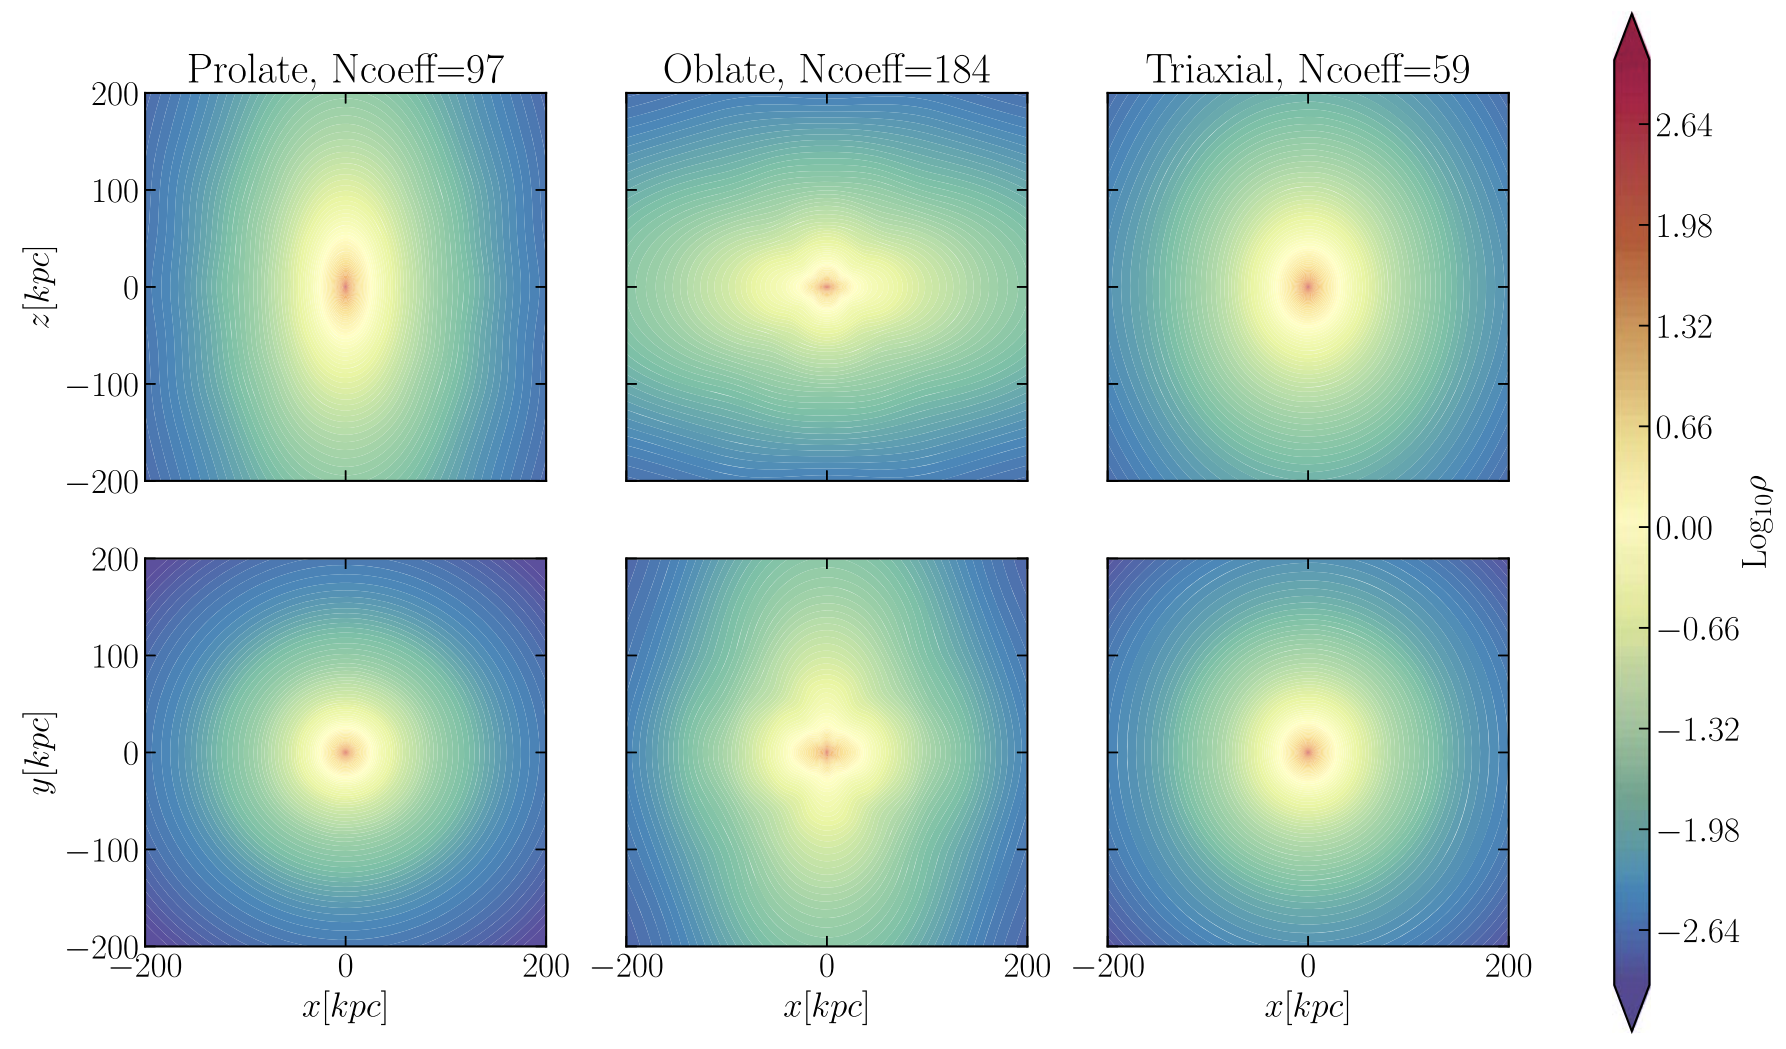
\includegraphics[width=\columnwidth]{2D_halo_shape.png}
    \caption{Ideal shapes and contour lines of the ideal shapes of the 2D projection.}
    \label{fig:shapes}
\end{figure}
These will be more precisely defined in section \ref{Method}. Unfortunately, simulations have not yet been successful in concluding whether or not our models of the DM halos reflect any of the ideal shapes. As of now, the simulations show halos which are too chaotic to accurately constrain. Although much more is being learned about the importance of halo shape there is still a lot of work to be done to understand the details of the galaxy-halo relationship. 


One of the most important questions surrounding the investigation of DM halo shape is how it might contribute to the structure of the baryonic matter within a galaxy. An excellent example of the significance of halo shape comes from \cite{Law10} in which a triaxial DM halo is constructed for the MW using the tidal debris from the nearby dwarf galaxy Sagittarius. This particular halo structure satisfies the tidal debris streams observed for Sagittarius as well as it's orbital path \citep{Law10}. This alone highlights the importance of halo shape however in response to this investigation \cite{Debattista_2013} used the triaxial shape of the MW halo to try and explain the disk structure of the MW. Although not entirely successful in reproducing a disk that fit the exact model, the team did observe some orientations of the disk which were supported by the triaxial halo. Other astrophysicists, such as Dr. Gurtina Besla, suspect new models could include the LMC which might correct for the gravitational potential along the intermediate axis and in turn support the observed MW disk structure. As whole, research into the shape of DM halos is illuminating for many reasons. Using observations of baryonic matter inform us of the structure of the DM halo and in turn how it might affect the galaxy it surrounds. Once the halo structure is resolved it can be used to investigate other features of the baryonic matter which either supports or changes the ideas about the predicted shape. The research into the MW-Sagittarius system is quite similar to how the shape of M33 might influence the structure of M31 and the evolution of the local group. Understanding the dramatic changes to M33's shape as the MW and M31 collide could offer insight into how the shape of the halo influences the baryonic structure of M31. This, in turn, motivates the research into M33 DM halo shape. 


\section{Shape of the M33 Dark Matter Halo}
This research paper focuses on the evolution of the dark matter halo of M31's most massive satellite galaxy, Triangulum (M33). More specifically, the research will investigate the tidal effects from the collision of MW \& M31 and how it contributes to the evolution of M33's dark matter halo. The primary structural feature which this report will explore in depth is the shape of the halo. Simulations of the MW-LMC system show that prolate, oblate, and triaxial shapes have different effects on the the baryonic matter of the galaxy. Additionally, as shown by \cite{Law10} and \cite{Debattista_2013}, the halo shape could have a lot of influence on the structure of the host halo. Unlike the previous research, the focus of this analysis will be on the evolution as the MW and M31 evolve towards a collision event approximately 11 Gyr. The reason for this specification is that the Local Group will undergo very dramatic changes as the system evolves.     


This research focuses on the effects of the tidal forces from the MW-M31 collision and how it changes the shape of the M33 halo. This is reminiscent of the research conducted by \cite{Law10} in which the shape of the MW is calculated using the tidal debris from the nearby dwarf galaxy Sagittarius. In this case the system will have a much larger gravitational potential due to the fact that the MW and M31 are much larger than the dwarf galaxy alone. This likely will produce more dramatic changes to M33's shape. Although not the focus of this inquiry, the halo shape might help predict how the baryonic matter of both M33 and it's host halo, M31, will evolve over time. Ideally, this will help the future modelling of DM in the local group and improve our understanding of DM. 


The importance of the research into M33's halo shape is shown clearly by researchers \cite{Law10, Debattista_2013, Garavito-Camargo_2021} whom all show significant impacts and changes to the observable baryonic matter in our Local Group due to halo shape. \cite{Law10} showed that tidal debris from a dwarf galaxy can help construct the shape of the MW DM halo. \cite{Debattista_2013} took that information and tried modelling how this shape fit into our current understanding of the MW disk. \cite{Garavito-Camargo_2021} showed that there could be an important relationship between halo shape and the dynamical friction wake of the LMC. All of these investigations are immensely important when trying to understand galactic evolution. They all show that the shape of DM halo could have very dramatic impacts on the galaxies and how they involve. However, all of these investigations have been focused directly on the MW system. Of course, this is very important considering we live in the MW and can most easily observe systems close by. However, research into the M31-M33 system is important within itself and might also help us draw conclusions about our own galaxy. By observing how M33's shape evolves during the collision event that will take place in the future could help inform us of what sort of things to look for when analyzing galaxies and how they evolved. Modelling the DM shape of M33 and how it is effected by tidal forces over time will show how it impacts the structure of it's own baryonic matter as well as M31. This could offer insight into what sort of things scientists might want to try and look for in our known universe to help model both DM and galactic evolution. 


\section{Methodology} \label{Method}
\subsection{Simulation}
The analysis of M33's halo shape will be completed using the N-body simulations ran by \cite{vdm12}. This simulation was constructed using N-body smoothed hydrodynamics code GADGET-3 \citep{Springel_2005}. N-body simulations can be described as a system of N particles in which the equations of motion are solved according to gravitational interaction \citep{Trenti08}. They are especially relevant to astrophysical models of our universe. They can play an important role in understanding a range of systems such as our solar neighborhood and even the local group.
\subsection{Design}
To understand the shape of the dark matter halo I constructed a plot of the halo using the composition of DM particles. Although current computational methods allow for a 3D projection of the halo it is very difficult to resolve any sort of shape using this representation. A 3D projection can provide reasonable insight into the structure of the halo but to accurately analyze the halo shape a series of 2D projections is much more efficient to measure the dimensions of the halo. One important reason 2D projections are more useful in determining the halo shape is that DM halos are very, very large structures which extend far beyond even galactic scales. As a result, the plot of the DM particles will encompass particles that are far beyond a reasonable distance in which the halo shape can be estimated. The shape is better represented by halos closer to the center of the halo. The region of interest can be estimated using the Jacobi radius of the halo. This was inspired by previous research into the structure of DM halos as shown by Figure \ref{fig:density_code} \citep{Chua22}.
\begin{figure}
	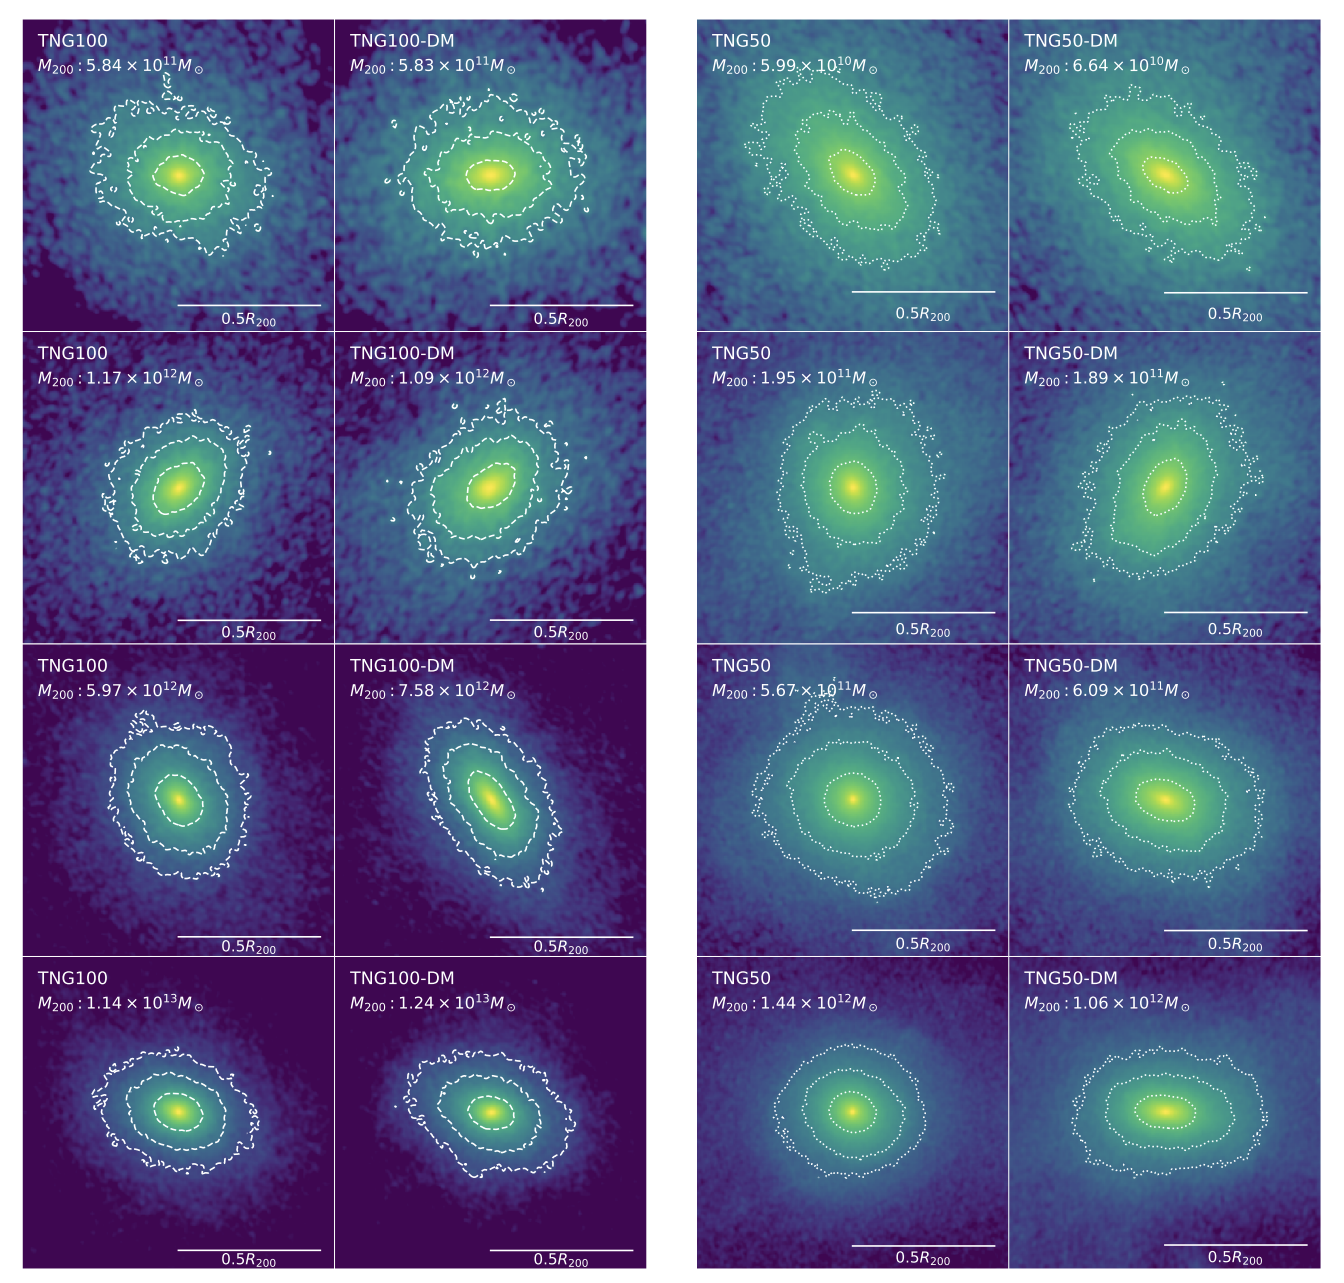
\includegraphics[width=\columnwidth]{density_countours.png}
    \caption{Example of the piece of code which creates a 2D density contour diagram}
    \label{fig:density_code}
\end{figure}
Figure \ref{fig:density_code} shows a series of 2D density plots of two halos. Contour lines are fitted to the density plots which represent regions with the same density of DM particles. I will use this method to analyze the structure of DM halos with a few slight modifications. First, the halos in Figure \ref{fig:density_code} show the halo with an inclination. To better capture the halo shape, I will rotate the halo such that it is oriented perpendicular to the z-axis. This will allow me to define the ellipsoidal axes for shape characterization. Additionally, I will fit contour line that encompasses particles within the Jacobi radius, as this region dictates the halo shape. Finally, I will create a covariance ellipse that will be fitted to the contour line of interest in order to define semi-major, semi-minor, and intermediate axes of the ellipsoid. The axes of the ellipsoid will be used to determine the shape of the halo. The halo will be characterized as either, triaxial, prolate, or oblate.
\subsection{Calculations}
Using the covariance ellipse, the semi-minor axis (z-axis) is defined as $c$, the semi-major axis (x-axis) is defined as $a$, and the intermediate axis (y-axis) is defined as $b$. I'll use the following equation given by \cite{Garavito-Camargo_2021} to characterize the shape of the halo.
\begin{equation} \label{shape_eq}
    T_{qs} = \frac{1-q^2}{1-s^2}
\end{equation}
The minor to major axis ration is defined by $s_\rho = c/a$ and the intermediate-to major axis ratio is defined by $q_\rho = b/a$. The value $T_{qs}$ is known as the triaxality of the halo. If $T_{qs} \ge 0.67$, the halo is a prolate ellipsoid. If $0.67 \ge T_{qs} \ge 0.33$, the halo is triaxial. If $T_{qs} \le 0.33$, the halo is oblate. A visual representation of the ideal shapes is given by Figure \ref{fig:shapes}.

\subsection{Plots}
Using the methodology outlined in the previous sections, I'll create 3 plots which aim to characterize the shape of the halo as the MW-M31 collision event evolves over time. These will be 2D density plots with contour lines that are fitted according to the density of DM particles. The inner most contour line will be defined using the Jacobi radius of the halo. A covariance ellipse will be matched to the innermost contour line so that the axes of the ellipsoid can be defined to calculate the dimensions of the shape. According to equation \ref{shape_eq} the shape of the halo will be characterized as triaxial, prolate, or oblate. Because I am interested in how the halo shape changes over the period of the collision event, I'll plot the shape during the pericenter and apocenter approach of M33 to M31. This is due to the fact the most dramatic changes to the structure will occur at these times and thus an accurate representation of the structural evolution can be analyzed. 


\subsection{Hypothesis} \label{hypo}
I predict that at the start of the simulation the shape of the M33 halo will be triaxial. I suspect that in addition to having a traxial shape the halo will also be spheroidal $(a=b=c)$. As the simulation progresses and the collision event between the MW \& M31 gets closer I think the tidal effects due to gravity will cause M33 to elongate and become prolate or oblate, depending on the orientation of the satellite in comparison to the MW-M31 merger. I think this will occur because the gravitational influence from the tidal effects of the combined MW-M31 system will become much stronger as they collide.   

\section{Results}
\begin{figure}
	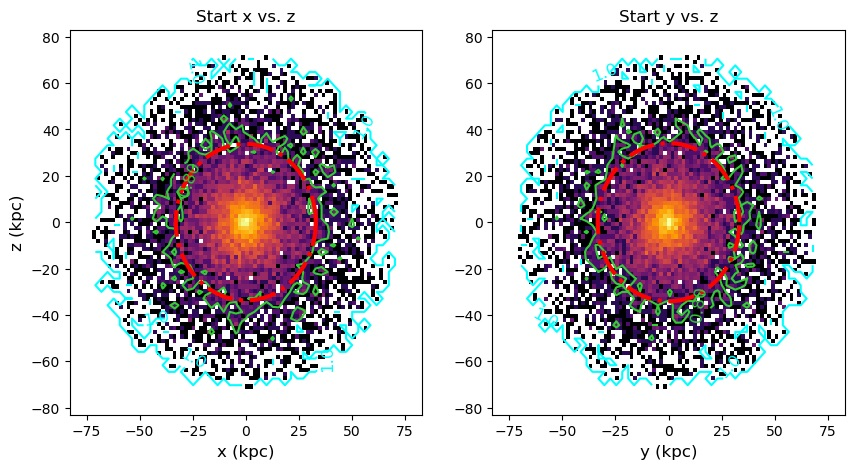
\includegraphics[width=\columnwidth]{starting_shape.jpeg}
    \caption{Starting shape of the M33 halo at a distance of 201 kpc and a jacobi radius of 73 kpc.}
    \label{fig:start}
\end{figure}


Figure \ref{fig:start} shows the starting shape of the M33 at snapshot zero. At this time, M33 is 201 kpc from M31. The jacobi radius at this time is 73 kpc. The plot of the halo only focuses on the particles within the jacobi radius because this region is the best representation of the shape of the halo. According to the definition of the halo shape provided by \cite{Garavito-Camargo_2021}, the halo is triaxial. This shape was defined using a density contour line which encompasses 80\% of the particles within this region. The triaxial shape of the halo is nearly spheroidal. This shape is very similar to the results found by \cite{Law10} in which the MW halo is triaxial in response to the Sagittarius tidal debris. According to the results of \cite{Law10} the triaxial shape of the halo influences the structure of M33. Additionally, the triaxial shape of the halo most likely influences the evolution of M31 and it's baryonic matter as indicated by \cite{Debattista_2013}.  

\begin{figure}
	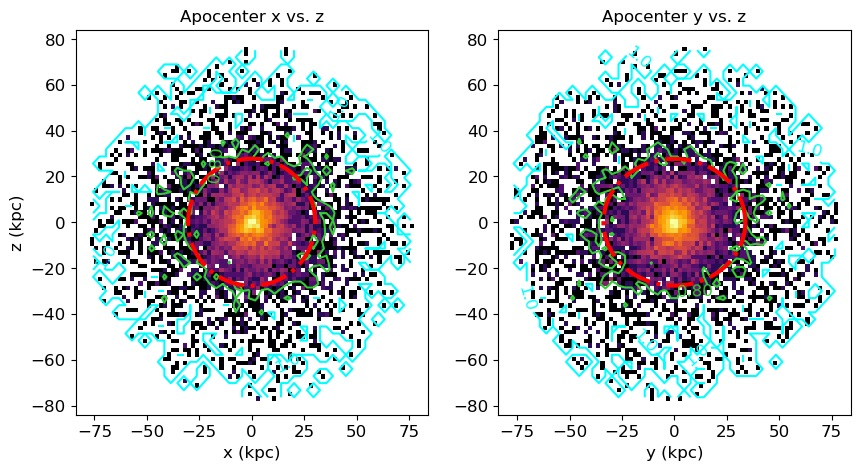
\includegraphics[width=\columnwidth]{apocenter_shape.jpeg}
    \caption{Apocenter shape of the M33 halo at a distance of 219 kpc and a jacobi radius of 79 kpc.}
    \label{fig:apocenter}
\end{figure}


Figure \ref{fig:apocenter} shows the shape of the M33 halo during the apocenter approach to M31. This is important because the apocenter approach will represent one of the most dramatic affects of the tidal forces on M33 during the evolution of the local group. The apocenter approach occurs at about 2.643 Gyr, at a distance of 219 kpc, and has a jacobi radius of 79 kpc. Again, the jacobi radius is the best indication of the halo shape as it evolves within the local group. Interestingly, although the apocenter approach is the furthest M33 will be from M31, it as apparent the effects from the tidal forces have already began. The halo changes from the initial triaxial shape to an oblate halo. This means the halo has been gravitationally influenced along the x-y axis. It should be noted the distance and jacobi radius do not seem to undergo changes that are dramatically different from the starting values. This is apparent in the 2D projection of the shape of the halo. Although it seems the density of particles has decreased, the shape of the shalo has changed.  

\begin{figure}
	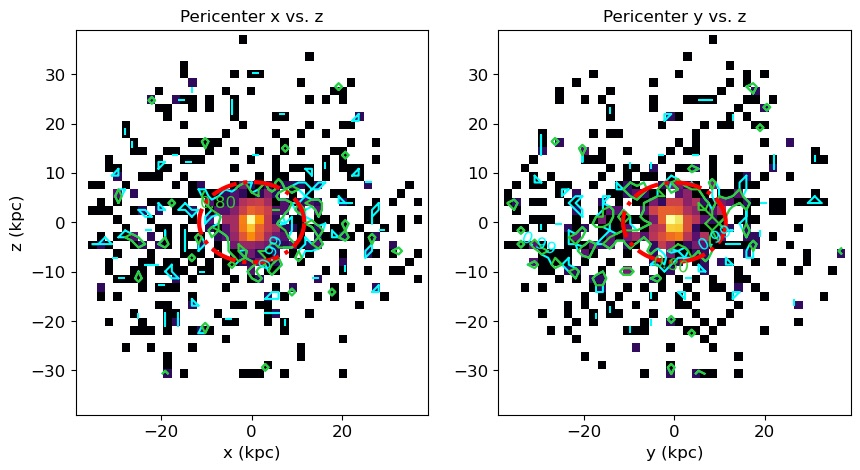
\includegraphics[width=\columnwidth]{pericenter_shape.jpeg}
    \caption{Pericenter shape of the M33 halo at a distance of 53 kpc and a jacobi radius of 19 kpc.}
    \label{fig:pericenter}
\end{figure}

Figure \ref{fig:pericenter} exhibits the most substantial changes to the M33 shape during the evolution of the local group. The pericenter approach occurs at around 11.357 Gyr, at a distance of 53 kpc, and has a jacobi radius of 19 kpc. Clearly, as the MW and M31 near each other, the tidal effects have a much greater impact. Although the halo still has an oblate shape like the apocenter approach, it is much more extended than previously. This is also shown by the fact that the density of particles dramatically decreases during the pericenter approach. This suggests the tidal effects of the collision event is the most influential during the pericenter approach. The shape of the M33 will significantly change from the starting shape as it moves towards the pericenter approach to M31 as the Local Group evolves.  

\section{Discussion}
As shown by the starting, apocenter, and pericenter shapes of the M33 DM halo, the tidal forces during the evolution of MW-M31 collision event dramatically influence the structure of M33. As the system evolves from the starting time until the pericenter time, approximately 11 Gyr later, the M33 halo shape changes from being triaxial to extremely oblate. The oblateness of the halo becomes more extended during the transition from the apocenter approach to the pericenter approach. This result does not reflect the exact hypothesis proposed in section \ref{hypo} however it comes very close. The starting halo shape was triaxial but not spheroidal. A closer look at the radii values revealed the halo was very close to being exactly spheroidal but was not. The evolution of the halo as the collision event occurred did match the predicted outcome. The gravitational influence from the tidal forces of MW-M31 stretched the halo along the x-y axes causing it to become oblate. This affect was most clearly seen during the pericenter approach which is not surprising considering at this time the MW and M31 have merged. It follows that there would be an immense gravitational influence from the merged system and thus it is likely this is what caused the oblateness of the halo. It should be noted that the calculations in this analysis do not account for the changes in mass of the M33 halo or M31. It also does not include the merger mass later on in the simulation. This could potentially influence the results and could be something that is accounted for in the future.  

Previous research indicates this change could have noticeable impacts on the structure of the baryonic matter of both M33 itself as well as it's host halo, M31. Extrapolating some of the conclusions from previous research done by \cite{Law10, Debattista_2013, Garavito-Camargo_2021}, it can be concluded changes to the shape of the M33 DM halo will impact on the baryonic structure of the entire Local Group. It is likely that transitioning from a triaxially shaped halo to a very oblate halo will cause the disk to reshape it's structure as shown by \cite{Debattista_2013}. Using the results of this research into the shape of M33 could help educate us on the tidal debris originating from the collision of the MW and M31 as shown by \cite{Law10}. The information from tidal debris can improve future models of how dark matter effects galactic evolution. Astrophysicists could also use the results of this simulation to help inform cosmological observations as it could give insight into what to look for when analyzing galaxy evolution. In addition, considering this investigation used the shape calculation derived by \cite{Garavito-Camargo_2021}, further analysis on the relationship between the shape of the halo and how it effects the Local Group system might illuminate the effectiveness of using this model.

This investigation which analyzes the shape of the M33 DM halo has offered promising results. It has illuminated the impacts of the tidal forces on the DM halo shape and offers great insight into the properties of galactic evolution. More refined methods of this research could improve the findings and could help develop better models for not only DM but also the halo-galaxy relationship during evolution.  

\section{Acknowledgements}
Immense appreciation is owed to Dr. Gurtina Besla and T.A. Hayden Foote. These two have guided this research from beginning to end and without their help it would not have been possible. They offered brilliant perspectives that vastly improved the quality of both the code and paper. Thank you. 

\bibliographystyle{mnras}
\bibliography{RA_2_references} 



% Don't change these lines
\bsp	% typesetting comment
\label{lastpage}
\end{document}

% End of mnras_template.tex
